\documentclass[]{beamer}
\usetheme{KUL}
\usepackage{multirow}
\usepackage{multicol}
\usepackage{tikz}
\usepackage{ulem}
\usepackage{todonotes}
\usepackage{siunitx}
\newcommand\itemS{\item[\textbf{\S}]}
\definecolor{darkgreen}{rgb}{0,0.598,0.199}
\usepackage{times} % set font on times new roman
\usepackage{eurosym} % package for Euro sign
\usepackage{lineno}   % package for line numbering
\usepackage{hyperref} % this is for url links
\usepackage{subcaption}  % this package enables one to put several figures next to each other
\usepackage{textcomp}
\usepackage{setspace}
\usepackage{gensymb}
\usepackage{tikz}
\usetikzlibrary{positioning}
\usetikzlibrary{matrix, arrows, graphs}
\usetikzlibrary{backgrounds}
\usetikzlibrary{calc}
\usepackage{amsmath}
\usepackage{adjustbox}
\usepackage[absolute,overlay]{textpos}


\usepackage[backend=biber,style=alphabetic]{biblatex}
\addbibresource{bibfile.bib}

\title{Secure boot, trusted boot and remote attestation for ARM TrustZone-based IoT Nodes}
\subtitle{Zhen Ling, Huaiyu Yan, Xinhui Shao, Junzhou Luo, Yiling Xu, Bryan Pearson,
Xinwen Fu \\ Journal of Systems Architecture 119 (2021)}
\author{Oberon Swings}
\institute{KU Leuven}
\date{\today}


\setbeamercolor{framesource}{fg=gray}
\setbeamerfont{framesource}{size=\tiny}
\newcommand{\source}[1]{\begin{textblock*}{0.4\textwidth}(0.75\textwidth ,0.8\textwidth)
    \begin{beamercolorbox}[ht=0cm,right]{framesource}
        \usebeamerfont{framesource}\usebeamercolor[fg]{framesource} {#1}
    \end{beamercolorbox}
\end{textblock*}}



\begin{document}

{
		\setbeamertemplate{headline}{} %define local, empty header for title page
		\setbeamertemplate{footline}{} %define local, empty footer for title page
		\source{\cite{article}}
		\maketitle
	}
	\addtocounter{framenumber}{-1} % We don't count the title page
	
\iftrue
% Table of Contents
\begin{frame}{Outline}
	\hfill	{\large \parbox{.95\textwidth}{\tableofcontents[hideothersubsections]}}
\end{frame}
\fi

\section{Introduction}

\begin{frame}{Goals}
\begin{itemize}
%The goal of this paper is to increase security in IoT devices which have an ARM chip with TrustZone.
\item IoT devices
\item ARM (TrustZone)
%The security is increased by checking the integrity of code running on the device during boot and execution.
\item Assure integrity
%Using their techniques they are able to defend against hardware, OS/firmware and software attacks.
\item Defend against \begin{itemize}
\item Hardware attacks
\item OS/Firmware attacks
\item Software attacks
\end{itemize}
\end{itemize}
\end{frame}

\begin{frame}{Solutions}
\begin{columns}
\column{0.5\textwidth}
\begin{itemize}
%First of all they have a special booting strategy to make sure the integrity is guaranteed when the IoT devices booted succesfully.
\item Hybrid booting \begin{itemize}
%The secure world is booted using secure boot, to provide strong security guarantees.
\item Secure boot
%The normal world is booted in a trusted manner, this way of booting is less strict than the secure boot but still provides a secure starting point for secure execution.
\item Trusted boot
\end{itemize}
%The IoT device is not necessarily safe after it has been booted, adversaries can still try to modify code while the device is operating. This is why the integrity of the processes needs to be measured.
\item Process integrity measurement \begin{itemize}
%These measurements are used to attest the processes in a pagebased way.
\item Pagebased attestation
\end{itemize}
\end{itemize}
\column{0.7\textwidth}
\begin{figure}
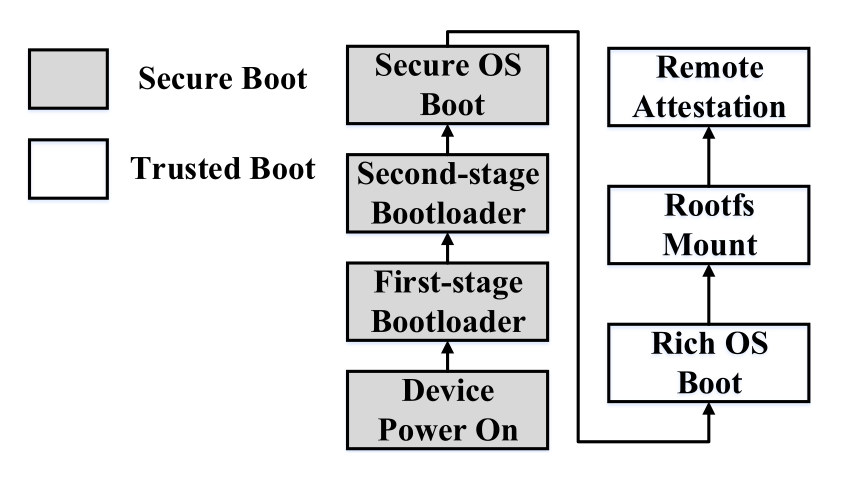
\includegraphics[width=1\textwidth]{Pictures/hybrid_boot.png}
\end{figure}
\end{columns}
\source{image: \cite{article}}
\end{frame}

\section{Hybrid booting}

\begin{frame}{Secure boot}
\begin{columns}
\column{0.5\textwidth}
\begin{itemize}
%Secure boot starts with an offline phase where the image of an application is measured. This measurement is hashed and this hash is signed to make sure the measurement is not tampered with.
\item Offline phase \begin{itemize}
\item Measure image
\item Hash
\item Sign
\end{itemize}
%During the actual secure boot the public key is verified, when this succeeds the public key is used to decrypt the signature. This decrypted signature can be used to compare with the hash of the image that the current module is trying to start.
\item Secure boot phase \begin{itemize}
%The first-stage bootloader is the first module that is started when booting, this is seen as the trusted base which uses a hardware Root of Trust.
\item First-stage bootloader trusted base
%Every module in the secure world locates the next module that needs to be loaded into memory and executed. When this module is found it is verified and only after succesful verification it is given control.
\item Locate next
\item Verify
\end{itemize}
\end{itemize}
\column{0.7\textwidth}
\begin{figure}
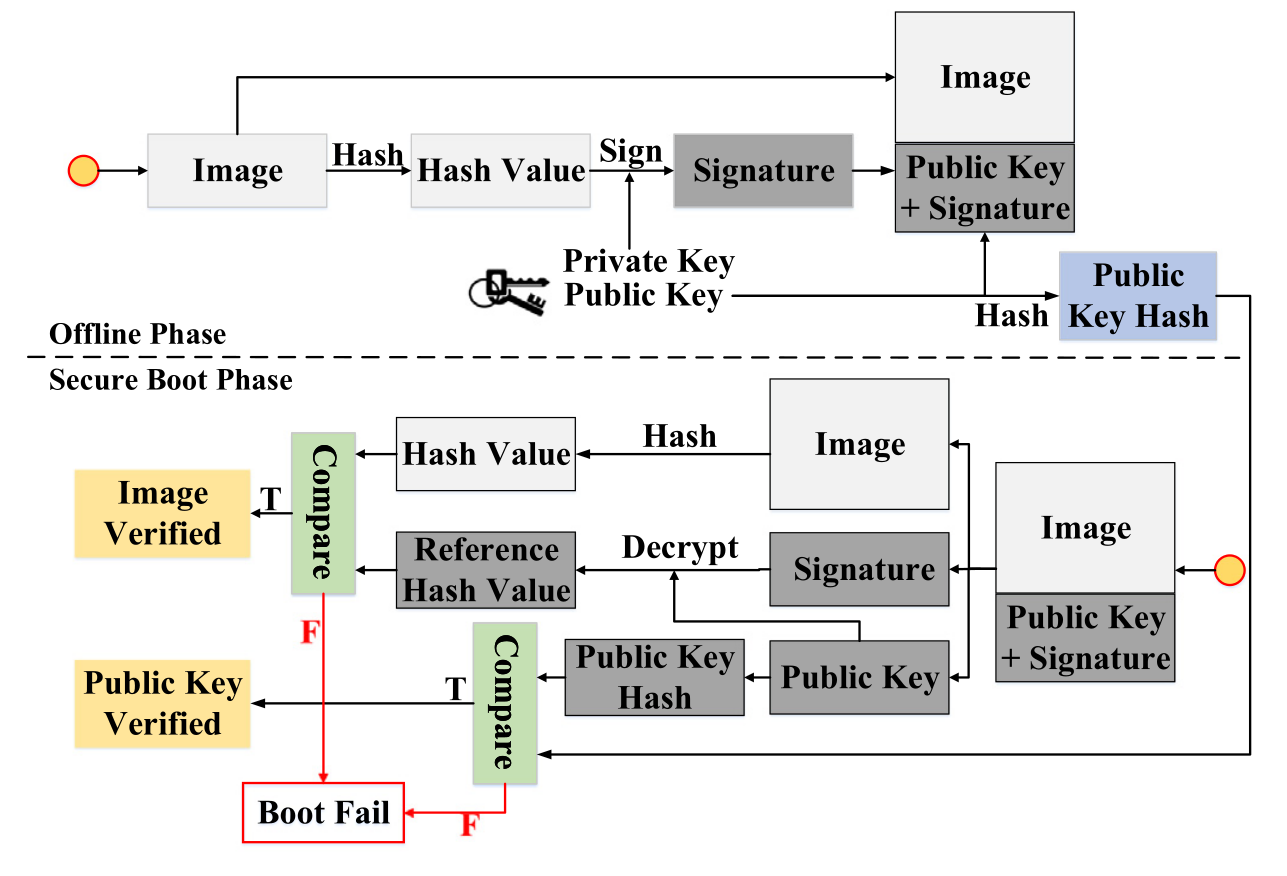
\includegraphics[width=1\textwidth]{Pictures/secure_boot.png}
\end{figure}
\end{columns}
\source{image: \cite{article}}
\end{frame}

\begin{frame}{Trusted boot}
\begin{columns}
\column{0.5\textwidth}
\begin{itemize}
%The trusted boot is less strict, it uses the hashes of the image to attest to a remote server that their integrity is not violated, but the booting process doesn't halt if this is not the case.
\item Offline phase \begin{itemize}
%Again the offline phase makes the initial measurements with which will be compared in the actual boot phase. These measurements are encrypted with a symmetric key and the encrypted text is stored on the remote attestation server.
\item Calculate hash
\item Encrypt with symmetric key
\item Store
\end{itemize}
%During the trusted boot phase the client application establishes a TLS connection with the verifier, and requests a nonce. The Cryptographic Acceleration and Assurance Module is used to recover the attestation key which is used to encrypt the nonce and the hash value. This encrypted text is send back to the verifier which checks the hash and the nonce to verify integrity and detect replay attacks respectively.
\item Trusted boot phase \begin{enumerate}
\item TLS connection nonce
\item Encrypt nonce \& hash
\item Respond
\item Hash verification (integrity) \\ Nonce verification (replay)
\end{enumerate}
\end{itemize}
\column{0.7\textwidth}
\begin{figure}
\centering
   \begin{subfigure}[b]{1\textwidth}
   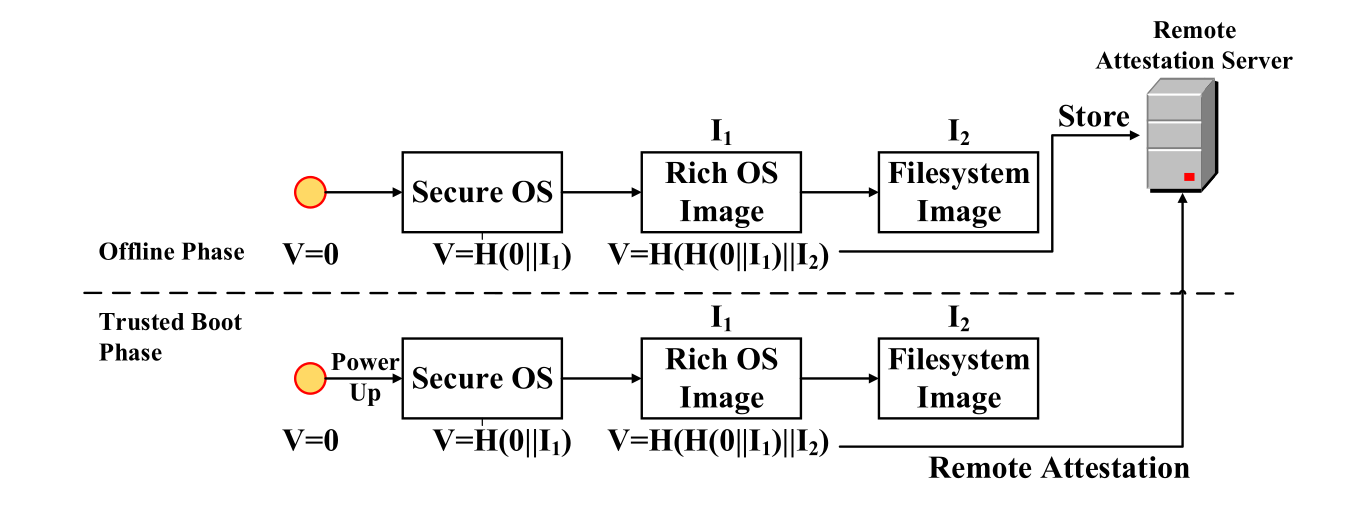
\includegraphics[width=1\textwidth]{Pictures/trusted_boot.png}
\end{subfigure}

\begin{subfigure}[b]{1\textwidth}
   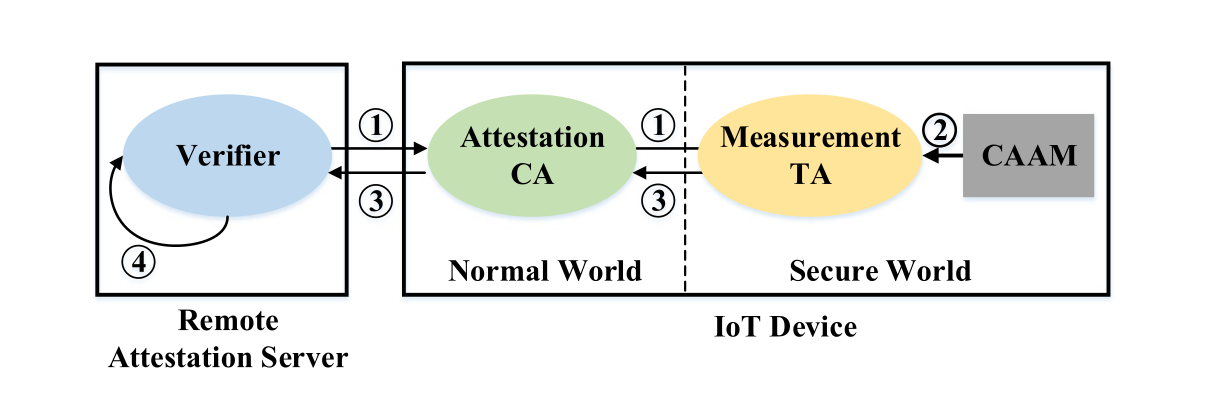
\includegraphics[width=1\textwidth]{Pictures/trusted_boot_attestation.png}
\end{subfigure}
\end{figure}
\end{columns}
\source{images: \cite{article}}
\end{frame}


\begin{frame}{Trusted boot encryption}
\begin{columns}
\column{0.7\textwidth}
\begin{itemize}
%A symmetric key is used as the attestation key, it can be assumed that this key is safe at the attestation server but the IoT device also needs access to this key without leaking it.
\item Symmetric key
\item Safe at server
%The IoT device generates a blob key using a random number generator. The attestation key is encrypted using this blob key and and MAC tag is added. The Cryptographic Acceleration and Assurance Module derives a Blob Key Encryption Key using the Master Key. The blob key is generated by concatenating these parts and the Master Key is stored in Secure Non-Volatile Storage. 
\item Storage in IoT device \begin{itemize}
\item Generate blob key (RNG)
\item Encrypt and MAC
\item Derive BKEK using MK
\item Concatenate parts
\item SNVS for Master Key
\end{itemize}
\end{itemize}
\column{0.5\textwidth}
\begin{figure}
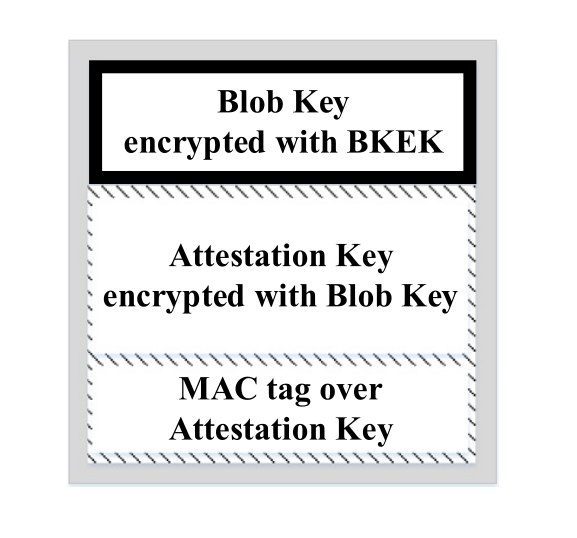
\includegraphics[width=1\textwidth]{Pictures/trusted_boot_encryption.png}
\end{figure}
\end{columns}
\source{image: \cite{article}}
\end{frame}

\section{Process integrity measurement}

\begin{frame}{Idea}
\begin{itemize}
%The secure boot makes sure the secure world can be used as a secure base for the trusted boot and attestation.
\item Secure boot base
%After the trusted boot it is attested that the programs integrity is not violated, of course this could still happen during runtime.
\item Runtime integrity 
%This is why all the code pages are measured using a trusted application. These measurements are then sent to a remote attestation server to provide the verifier with proof that the processes running on the IoT device are not tampered with.
\item Measure code pages
\item Measurement TA
\item Remote Attestation Server
\end{itemize}
\end{frame}

\begin{frame}{Process integrity measurement}
\begin{columns}
\column{0.5\textwidth}
\begin{enumerate}
%TA maps physical address of init_task into the virtual address space of the SW. 
\item Map address of init\_task
%The measurement TA obtains the physical address by subtracting the standard offset between virtual and physicall addresses.
\item Obtain physical address
%The physical address is transformed into the corresponding SW virtual address.
\item Transform to virtual address
%The measurement TA calculates the page boundaries.
\item Calculate page boundaries
%Finally the measurement TA measures each page of the process.
\item Measure each page
\end{enumerate}
\column{0.7\textwidth}
\begin{figure}
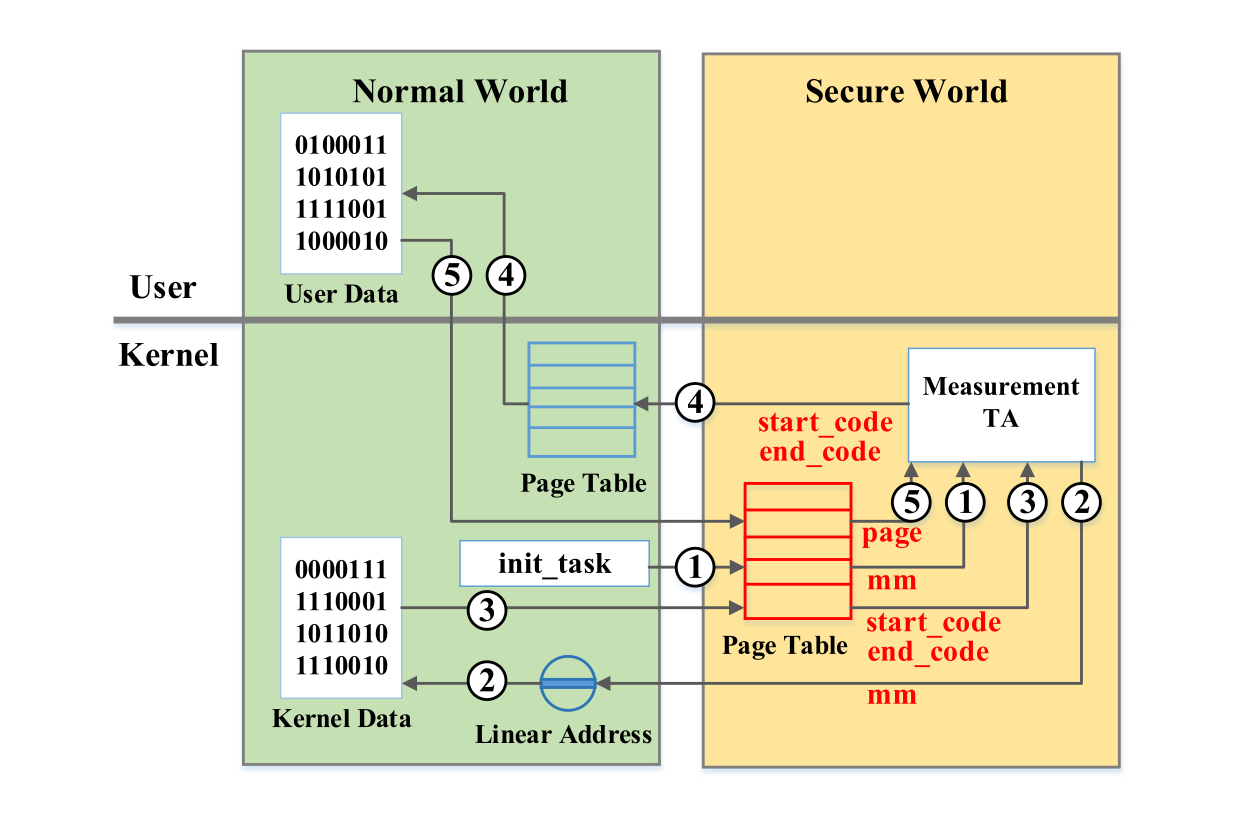
\includegraphics[width=1\textwidth]{Pictures/process_measurement.png}
\end{figure}
\end{columns}
\source{image: \cite{article}}
\end{frame}

\begin{frame}{Process integrity attestation}
\begin{columns}
\column{0.5\textwidth}
\begin{enumerate}
%After establishing a TLS connection with the verifier the attestation client application requests a nonce.
\item Request nonce
%The measurement TA measures the pages of the processes, the process described in the previous slide.
\item Calculate measurement
%The CAAM provides the attestation key which is used to encrypt the nonce and the measurement.
\item Encrypt attestation info
%If other processes need to be measured too these measurements need to be executed and appended to the current measurement list. If all processes have been measured the cyphertext is sent to the attestation client application.
\item Send cyphertext and \\ repeat 2 or continue
%The cyphertext is forwarded to the verifier which will check the nonces and measurements to detect new or modified software.
\item Send cyphertext to verifier
\item Verify (new, modified)
\end{enumerate}
\column{0.7\textwidth}
\begin{figure}
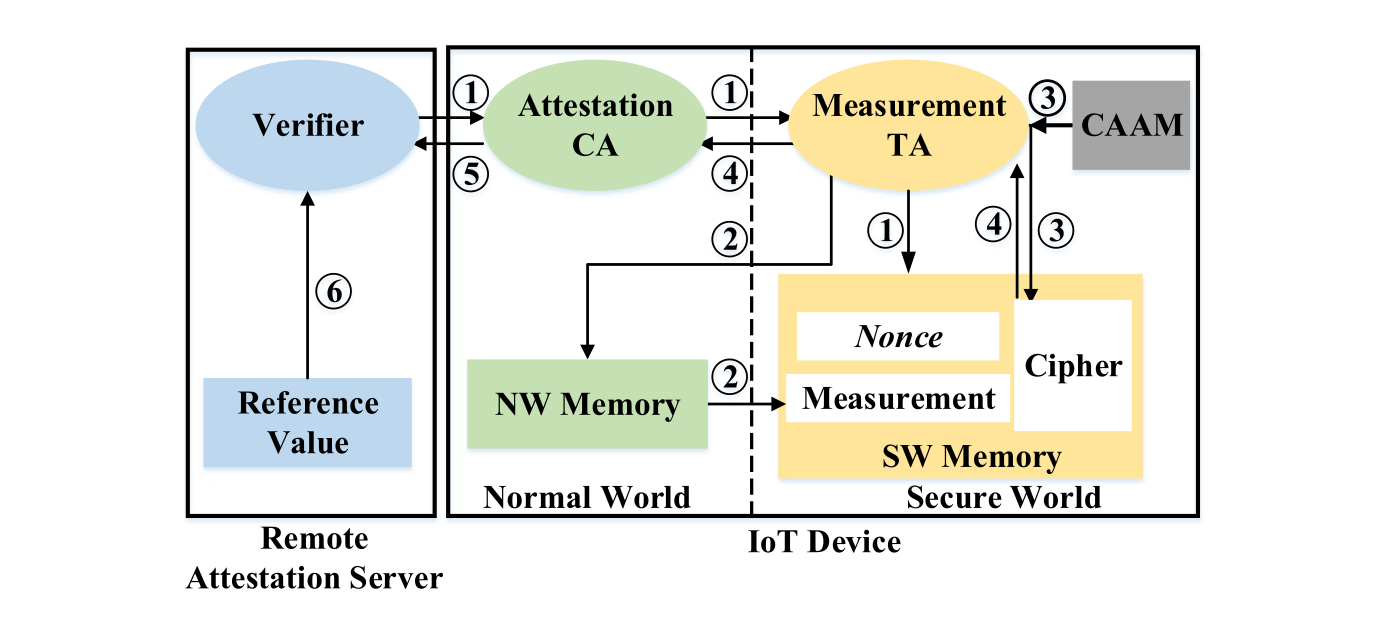
\includegraphics[width=1\textwidth]{Pictures/process_remote_attestation.png}
\end{figure}
\end{columns}
\source{image: \cite{article}}
\end{frame}

\section{Evaluation \& security analysis}

\begin{frame}{Results}
\begin{columns}
\column{0.5\textwidth}
\noindent\textbf{Performance}
\begin{itemize}
%It is rather obvious that secure boot adds overhead to the booting process because all the hashes need to be calculated and the keys need to be restored using private/public key cryptography.
\item Secure boot doubles secure OS boot-time
%The trusted boot is much more light weight because symmetric keys are used.
\item Trusted boot adds little overhead (0.5\%)
%The overhead of the measurement and attestation is given in a rather strange way. The overhead of running the attestation gives a range between half a percent negative to half a percent positive overhead which doesn't tell much. We think it would have been more meaningfull to provide details about how long attestation or measurement of x amount of pages of 2 kB takes, this gives more insight about how often it should be run to have a good balance between performance and security.
\item Measurement TA and attestation CA overhead (-0.5\% $\approx$ +0.5\%)
\end{itemize}
\column{0.5\textwidth}
\noindent\textbf{Security}
\begin{itemize}
%The secure boot provides a secure base because when the secure world is booted correctly the hardware isolation mechanism provided by ARM TrustZone ensures that the NW cannot compromise the SW where the measurement TA and the CAAM for encryption reside. 
\item Secure boot gives secure base
%The measurement method relies on the integrity of the NW linux paging structure and process management kernel objects. This method is vulnerable to malware capable of self-hiding but it is mentioned that this will be looked at in future work.
\item Measurement method relies on NW
\end{itemize}
\end{columns}
\end{frame}

\section{Relevance for thesis}

\begin{frame}{Focus shift}
\begin{itemize}
%The secure boot what we we're working on last time was mainly to get the device up and running with the trusted execution environment. This was harder than expected so we're back at working with the simulator but now we're focussing on implementing and researching academically relevant solutions.
\item Secure boot (engineering)
%The attestation is our main focus. We believe that the PinePhone could be turned into a secure open platform by having the SW attest the NW and inform the user (using secure IO) about possible threats.
\item Attestation \begin{itemize}
\item Informing user
\item Securing NW
\end{itemize}
%We start with reproducing the attestation method described in the paper. The process measurement should be very similar but for the attestation the remote attestation server will not be taken into account.
\item Reproduction \begin{itemize}
\item Process measurement
\item Process attestation
\end{itemize}
%A first adjustment is that we will not work with a remote server because we believe that user attestation is more appropriate in a smartphone environment. Secondly if there is time we'd like to work on the reliance on the NW OS for the measurement. The SW is able to inspect all NW memory and with this in mind we believe it should be feasible to do measurements without the NW having to provide addresses or memory access.
\item Adjustments \begin{itemize}
\item Remote server
\item Reliance on NW OS
\end{itemize}
\end{itemize}
\end{frame}

\begin{frame}{Differences}
\begin{columns}
\column{0.5\textwidth}
\noindent\textbf{Paper}
%The paper implemented secure and trusted boot while in this thesis we will assume a secure boot and won't look into the trusted boot. Secondly in the paper they used remote attestation while we will attest the NW using the SW and alert the user so some form of user attestation. Lastly the paper assumed pure IoT devices which don't install additional software or don't have regular software updates. In this thesis we look more at secure open platforms in the sense that software from multiple stakeholders should be able to run on the same platform and that this software is able to update or even more software being added shouldn't give any trouble.
\begin{itemize}
\item Secure boot
\item Trusted boot
\item Remote attestation
\item IoT devices
\end{itemize}
\column{0.5\textwidth}
\noindent\textbf{Thesis}
\begin{itemize}
\item Secure boot assumed
\item No Trusted boot
\item SW attests NW
\item Secure Open platform
\end{itemize}
\end{columns}
\end{frame}

\part{}

\begin{frame}{Questions?}
\begin{figure}

\includegraphics[width=0.7\textwidth]{Pictures/questions.jpg}
\end{figure}
\source{image: https://www.toonpool.com/cartoons/ Question\_376876}
\end{frame}

\begin{frame}[t]{References}
\printbibliography
\end{frame}


\end{document}